

\subsection{The  basket call option under the discretized multi-dimensional Black-Scholes}\label{sec:The basket option under time stepping framework}

In the following, I present two ways of solving the root finding problem in multi-dimension. The first way, presented in Section \ref{sec: First way},  is an extension of Section \ref{sec:The discretized 1D Black-Scholes}, and the numerical results in Section \ref{sec:Result for the  $2$-dimensional Basket call option} are based on applying this way of numerical smoothing. In the second way, presented in Section \ref{sec: Second way}, we tried a different approach that is inspired by  the work of \cite{bayersmoothing}. However, the way I did it, it seems to me that we do not  need numerical smoothing and the smoothing can be done analytically.

\subsubsection{First way}\label{sec: First way}
In this suggested way, I try to extend the way we solved the one dimensional problem, as in Section \ref{sec:The discretized 1D Black-Scholes}, to higher dimensions.

We consider the basket option under multi-dimensional BS model where the process $\mathbf{X}$ is the discretized $d$-dimensional Black-Scholes model and the payoff function $g$ is given by
\begin{align}
	g(\mathbf{X}(T))=\max\left(\sum_{i=1}^{d} \omega_{i} X^{(i)}(T)-K,0  \right)	
\end{align}
Precisely, we are interested in the  $d$-dimensional lognormal example where the dynamics of the stock are given by

\begin{align}\label{lognormal_dynamics_basket}
	dX^{(i)}_t=\sigma^{(i)} X^{(i)}_t dB^{(i)}_t,
\end{align}

where $\{B^{(1)}, \dots,B^{(d)}\}$ are correlated Brownian motions with correlations $\rho_{ij}$.


In the discrete case, the numerical approximation of $X^{(j)}(T)$ satisfies


\begin{align}
	\bar{X}^{(j)}_T&=\Phi(\Delta t, z_1^{(j)}, \Delta B^{(j)}_0,\dots,\Delta B^{(j)}_{N-1}),  \quad 1 \le j \le d, \\ \nonumber
	&=\Phi(\Delta t, \Psi(z_1^{(j)},\dots,z_N^{(j)})), \quad 1 \le j \le d,
\end{align}
for some path function $\Phi$ and Brownian bridge map $\Psi$ as described in Section \ref{sec:Brwonian bridge construction}.

Using results from section \ref{sec:The discretized 1D Black-Scholes}, we have

\begin{align}
	\bar{X}^{(j)}(T)=X_0^{(j)} \prod_{i=0}^{N-1} \left[ 1+\frac{\sigma^{(j)}}{\sqrt{T}} z^{(j)}_1 \Delta t+ \sigma^{(j)} \Delta B^{(j)}_{i}\right], \quad 1 \le j \le d.
\end{align}
Therefore, in order to determine $\mathbf{y}_{\ast}=(y_{\ast}^{(1)},\dots,y_{\ast}^{(d)})$, we need to solve
\begin{align}
	\mathbf{x}=\sum_{j=1}^{d} \omega_j X^{(j)}_0 \prod_{i=0}^{N-1} \left[ 1+\frac{\sigma^{(j)}}{\sqrt{T}} y^{(j)}_{\ast}(\mathbf{x}) \Delta t+ \sigma^{(j)} \Delta B^{(j)}_{i}\right],
\end{align}

which implies that the location of the kink point for the approximate problem is equivalent to finding the roots of the polynomial $P(\mathbf{y}_\ast(K))$, given by
\begin{align}\label{polynomial_kink_location_basket}
	P(\mathbf{y}_{\ast}(K))&=\sum_{j=1}^{d} \omega_j X^{(j)}_0 \prod_{i=0}^{N-1} \left[ 1+\frac{\sigma^{(j)}}{\sqrt{T}} y^{(j)}_{\ast} \Delta t+ \sigma^{(j)} \Delta B^{(j)}_{i}\right]-K, \nonumber\\
	&=\sum_{j=1}^{d} \omega_j X^{(j)}_0 \left(\prod_{i=0}^{N-1} \left[ 1+\frac{\sigma^{(j)}}{\sqrt{T}} y_\ast^{(j)} \Delta t+ \sigma^{(j)} \Delta B^{(j)}_{i}\right]-\frac{K}{ \omega_j X^{(j)}_0  d}\right) \nonumber\\
	&=\sum_{j=1}^{d} \omega_j X^{(j)}_0 P^{(j)}\left(y_\ast^{(j)}\left(\frac{K}{ \omega_j X^{(j)}_0  d }\right)\right)
\end{align}

Therefore, the problem of finding the kink in the $d$-dimensional problem is brought to finding the location of the kink for each dimension by solving the root of the polynomial $P^{(j)}\left(y_\ast^{(j)}\left(\frac{K}{\omega_j X^{(j)}_0 }\right)\right)$.  

Using  \textbf{Newton iteration method}, we use the expression $P'=\frac{d P^{(j)}}{d y_\ast^{(j)}}$. If we denote $f_i^{(j)}(y)=1+\frac{\sigma^{(j)}}{\sqrt{T}} y \Delta t+ \sigma^{(j)} \Delta B^{(j)}_{i}$, then we can easily show that
\begin{align}\label{polynomial_kink_location_derivative_basket}
	P'^{(j)}(y)=\frac{\sigma^{(j)} \Delta t}{\sqrt{T}} \left( \prod_{i=0}^{N-1} f_i^{(j)}(y)\right) \left[ \sum_{i=0}^{N-1} \frac{1}{f_i^{(j)}(y)}\right].
\end{align}




Therefore, in this case, the integrand $h(\mathbf{z}^{(1)}_{-1},\dots,\mathbf{z}^{(d)}_{-1})$ (as expressed in \eqref{eq: pre_integration_step_wrt_y1_basket}) is given by

\begin{align}\label{smoothed_integrand_basket_opt_2d}
	h(\mathbf{z}^{(1)}_{-1},\dots,\mathbf{z}^{(d)}_{-1})&= \int_{\Omega}  \max  \left[ \left(\sum_{j=1}^{d} \Phi \circ \Psi(T;z_1^{(j)},\mathbf{z}^{(j)}_{-1})\right)-K,0\right]   \rho_d(z_1^{(1)},\dots,z_1^{(d)}) dz_1^{(1)}\dots dz_1^{(d)}.
\end{align}


We get the kink point by running Newton iteration in each dimension seperately for root solving of each polynomial $P^{(j)}$ as expressed in \eqref{polynomial_kink_location_basket} with a precision of $10^{-10}$. We  decompose the total integration domain $\Omega$  into sub-domains $\Omega_i,\: i=1,2,\dots, 2^d$ such that the integrand is smooth in the interior of  $\Omega_i$ and such that the kink is located along the boundary of these areas. The total integral is then given as the sum of the separate integrals, \ie
\begin{align}
	h(\mathbf{z}^{(1)}_{-1},\dots,\mathbf{z}^{(d)}_{-1}) &:=  \int_{\Omega}  \max  \left[ \left(\sum_{j=1}^{d} \Phi \circ \Psi(T;z_1^{(j)},\mathbf{z}^{(j)}_{-1})\right)-K,0\right]   \rho_d(z_1^{(1)},\dots,z_1^{(d)}) dz_1^{(1)}\dots dz_1^{(d)}  \nonumber\\
	&=\sum_{i=1}^{2^d}	\int_{\Omega_i} 
	\max  \left[ \left(\sum_{j=1}^{d} \Phi \circ \Psi(T;z_1^{(j)},\mathbf{z}^{(j)}_{-1})\right)-K,0\right]   \rho_d(z_1^{(1)},\dots,z_1^{(d)}) dz_1^{(1)}\dots dz_1^{(d)},
\end{align}

where we use Gauss-laguerre quadrature with $\beta$ points to get each part.

\FloatBarrier


\subsubsection{Second way}\label{sec: Second way}
 The $i$-th asset $X^{(i)}$ of the basket $(i=1,\dots,d)$ is given by 

\begin{equation}
X^{(i)}_{k \Delta t}=X^{(i)}_0 \exp\left( -\frac{\sigma_i^2}{2} k \Delta t +\sigma_i B^{(i)}_{k\Delta t}\right), \quad 1 \le k \le N  \COMMA
\end{equation} 
where $X^{(i)}_0$ is the current price of the $i$-th asset, $\sigma_i$ is the volatility of the $i$-th asset and $B=(B^{(1)},\dots, B^{(d)})$ is a $d$-dimensional Brownian motion. The correlation between $B^{(i)}$ and $B^{(j)}$ is denoted by $\rho_{ij}$. The payoff function of the European basket option is given by 
\begin{equation}\label{eq:basket_call_payoff}
f(Z)=\max\left(\sum_{i=1}^{d} c_i X^{(i)}_T(Z) -K,0\right)\COMMA
\end{equation}
where $c_i$ is the corresponding weight of the $i$-th asset, $Z \in \rset^{N \times d}$ is standard Gaussian  vector, and 


\begin{equation}
X^{(i)}_{k \Delta t} (Z)=X^{(i)}_0 e^{-\frac{\sigma_i^2}{2} k \Delta t} \exp\left(\sum_{j=1}^{d  N} C_{(k-1) d +i,j} Z_j\right) \PERIOD
\end{equation}
where $C$ is a $dN \times dN$-matrix with $C C^T=\bar{\Sigma}:=R  \otimes \Sigma$ ($\Sigma$ is $N \times N$ matrix  given by \eqref{eq:covariance_matrix_in_time}), and $R$ is an $d \times d$-matrix with $R_{ij}=\sqrt{T/N} \rho_{ij} \sigma_i\sigma_j$. 

Therefore, we have

\begin{align}\label{eq:asset_dynamics_last_inc}
X^{(i)}_{T} (Z)=X^{(i)}_{N \Delta t}(Z)&=X^{(i)}_0 e^{-\frac{\sigma_i^2}{2} T} \exp\left(\sum_{j=1}^{d  N} C_{(N-1) d +i,j} Z_j\right) \nonumber\\
&=\tilde{w}^{(i)}  \exp\left(A_{i\ast} Z\right)\nonumber\\
&=\tilde{w}^{(i)}  \exp\left(\widetilde{Z}^{(i)}\right)\COMMA
\end{align}
where $\tilde{w}^{(i)}=X^{(i)}_0 e^{-\frac{\sigma_i^2}{2} T} $,  $A$ is a   $d \times dN$  matrix such that $A:=\left(C_{(N-1) d +i,j} \right)_{1 \le i \le d, \: 1 \le j \le dN }$,  $A_{i\ast}$ is the $i$-th row vector of A, and $\widetilde{Z}=AZ$.

Let us denote by $\widetilde{\Sigma}$ the covariance matrix of $\widetilde{Z}$, then $\widetilde{\Sigma}=A A^T$. If we use the same approach in \cite{bayersmoothing}, Specifically Lemma $3.1$, then we can write 
\begin{equation}
\widetilde{\Sigma}=\widetilde{V} \widetilde{D} \widetilde{V}^T
\end{equation} 

such that $\tilde{D}=\text{diag}(\lambda_1^2, \dots, \lambda_d^2)$ is $d \times d$ diagonal matrix and $\widetilde{V} \in \rset^{d \times d}$ is an invertibe matrix, with the property that $\widetilde{V}_{i,1} \equiv 1,\: i=1,\dots,d$.


Going back to \eqref{eq:basket_call_payoff}, and replacing $\widetilde{Z}$ by $\widetilde{V} Y$, such that  $Y:=\widetilde{V}^{-1} \widetilde{Z} \sim \mathcal{N}(0,\widetilde{D})$, we obtain

\begin{align}\label{eq:basket_call_payoff_2}
f(Z)&=\max\left(\sum_{i=1}^{d} c_i X^{(i)}_T(Z) -K,0\right) \nonumber\\
&=\max\left(\sum_{i=1}^{d} w^{(i)} \exp\left(\widetilde{Z}^{(i)}\right) -K,0\right) \nonumber\\
&=\max\left(\sum_{i=1}^{d} w^{(i)} \exp\left((\widetilde{V} Y)^{(i)}\right) -K,0\right) \nonumber\\
&=\max\left(\sum_{i=1}^{d} w^{(i)} \exp\left( Y_1+ \sum_{j=2}^{d}\widetilde{V}_{ij} Y_j\right) -K,0\right) \nonumber\\
&=\max\left(h(Y_2, \dots,Y_d) e^{Y_1} -K,0\right) \COMMA
\end{align}

where $w^{(i)}=c_i \tilde{w}^{(i)}$ and $h(y_2,\dots,y_d):= \sum_{i=1}^{d} w^{(i)} \exp\left(\sum_{i=1}^{d} w^{(i)}  \sum_{j=2}^{d}\widetilde{V}_{ij} Y_j \right)$. 


Giving  \eqref{eq:basket_call_payoff_2}, and Lemma $3.3$ in \cite{bayersmoothing}, it seems to me that we do not  need numerical smoothing and the smoothing can be done analytically using conditional expectation formula. 







%For notation simplification, let us denote  by $\mathbf{Z}^{(i)}:=(Z_{N(i-1)+1}, \dots, Z_{iN})$ and  $\mathbf{Z}^{(i)}_{-1}:=(Z_{N(i-1)+2}, \dots, Z_{iN})$. 


%Going back to \eqref{eq:basket_call_payoff}, we have 
%\begin{align}\label{eq:basket_call_payoff_2}
%	f(Z)&=\max\left(\sum_{i=1}^{d} c_i S^{(i)}_T(Z) -K,0\right) \nonumber\\
%	&=\max\left(\sum_{i=1}^{d} w_i \exp\left(\sum_{j=1}^{dN}C_{(N-1) d +i,j} Z_j\right) -K,0\right) \nonumber\\
%	&=\max\left(\sum_{i=1}^{d} w_i \left( \exp\left(\sum_{\ell=1}^{d}C_{(N-1) d +i,(\ell-1)N+1} Z_{(\ell-1)N+1}+\sum_{\underset{j \neq (\ell-1)N+1, 1\le \ell\le d} {j=1}}^{dN}C_{(N-1) d +i,j} Z_j \right)\right) -K,0\right) \nonumber \\
%	&=\max\left(\sum_{i=1}^{d} w_i \exp(y_i)  \exp\left(\sum_{\underset{j \neq (\ell-1)N+1, 1\le \ell\le d} {j=1}}^{dN}C_{(N-1) d +i,j} Z_j \right) -K,0\right)\nonumber\\
%	&=\max\left(\sum_{i=1}^{d} w_i \exp(y_i)  h_i( \mathbf{Z}^{(1)}_{-1}, \dots \mathbf{Z}^{(d)}_{-1})-K,0\right)
%	\COMMA
%\end{align}
%where
%\begin{align*}
%	w_i&=c_i X^{(i)}_0 e^{-\frac{\sigma_i^2}{2} T}\\
%	y_i&=\sum_{\ell=1}^{d}C_{(N-1) d +i,(\ell-1)N+1} Z_{(\ell-1)N+1}\\
%	h_i( \mathbf{Z}^{(1)}_{-1}, \dots \mathbf{Z}^{(d)}_{-1})&=	\exp\left(\sum_{\underset{j \neq (\ell-1)N+1, 1\le \ell\le d} {j=1}}^{dN}C_{(N-1) d +i,j} Z_j \right)\PERIOD
%\end{align*}
%
%$y_i$ can be seen always as a linear combination including the first factors in each asset dimension.




\subsection{Result for the  $2$-dimensional Basket call option}\label{sec:Result for the  $2$-dimensional Basket call option}
\subsubsection{Weak error plots} \label{sec:Weak error plots_Basket_2D_call}

We consider the case of $2$-dimensional Basket call option, with parameters: $S^{(1,2)}=100$, $K=100$, $\sigma^{(1,2)}=0.4$, $\rho=0.3$, $r=0$, $T=1$.  The MC  value of this case (with large number of samples) is $12.900784$ with a statistical error equal to $	0.001033$ (Provided by Premia).


In this section, we include the results of weak error rates for $2$ scenarios, without/with Richardson extrapolation (level $1$). We note that the weak errors plotted here correspond to relative errors.  

 We can see from figure \ref{fig:Weak_rate_basket_2d} that we get a weak error of order $\Delta t$ for the case without Richardson extrapolation and almost $\Delta t^2$ for the case with Richardson extrapolation. 
 
% From figure \ref{fig:Weak_rate_call_with_rich_level1_beta_64}, we observe an improvement in the rate and the constant when using level $1$ of Richardson extrapolation, approximately of order $\Delta t^2$. For all the plots below, the upper and lower bounds are $95\%$ confidence interval.



\begin{figure}[h!]
	\centering
	\begin{subfigure}{.35\textwidth}
		\centering
		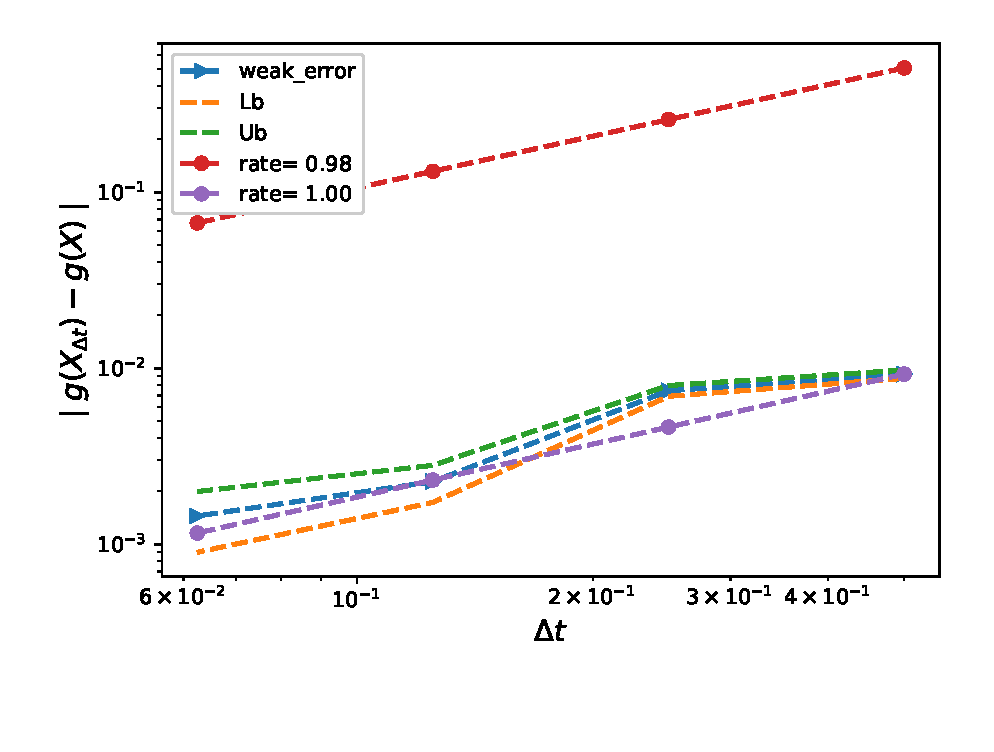
\includegraphics[width=1\linewidth]{./figures/weak_error_rates_basket_2d/without_richardson/weak_convergence_order_basket_option_2d_1_relative_M_4_10_7_plain}
		\caption{}
		\label{fig:sub3}
	\end{subfigure}%
	\begin{subfigure}{.35\textwidth}
		\centering
		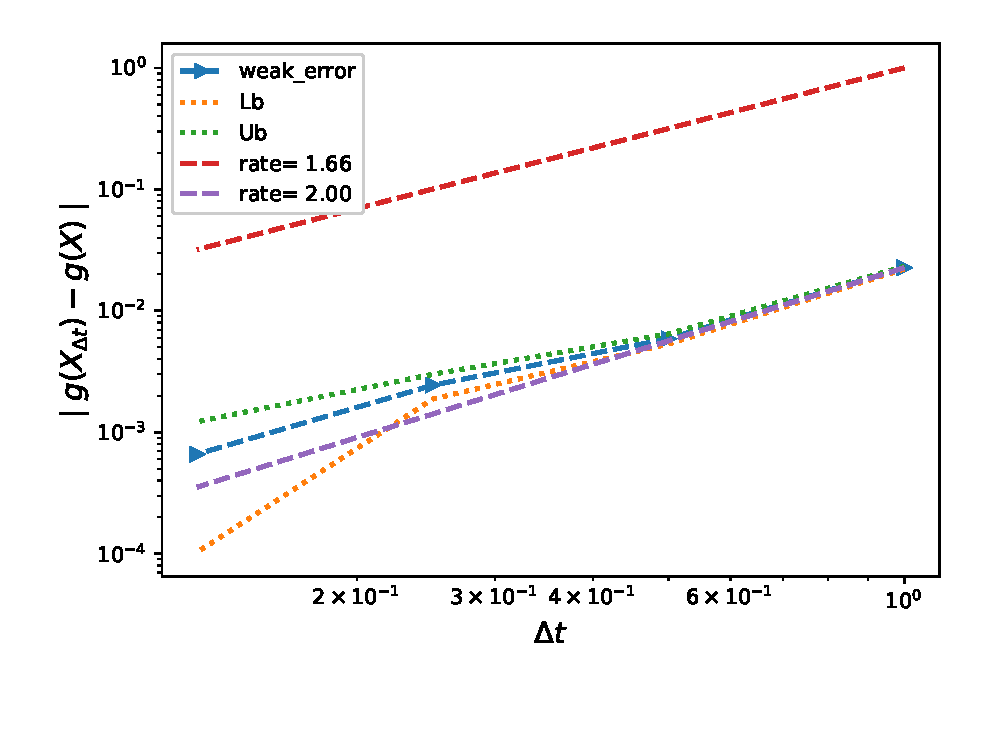
\includegraphics[width=1\linewidth]{./figures/weak_error_rates_basket_2d/with_richardson/weak_convergence_order_basket_option_2d_1_richardson_relative_M_4_10_7_plain}
		\caption{}
		\label{fig:sub4}
	\end{subfigure}
	
	\caption{The rate of convergence of the weak error for the Basket ($2$-dimensional) call option using MC. a) $\abs{\expt{g(X_{\Delta t})}-g(X)}$  b) $\abs{\expt{2 g(X_{\Delta t/2}) -g(X_{\Delta t})}-g(X)}$}
	\label{fig:Weak_rate_basket_2d}
\end{figure}






%\begin{figure}[h!]
%	\centering
%	\begin{subfigure}{.35\textwidth}
%		\centering
%		\includegraphics[width=1\linewidth]{}
%		\caption{}
%		\label{fig:sub3}
%	\end{subfigure}%
%	\begin{subfigure}{.35\textwidth}
%		\centering
%		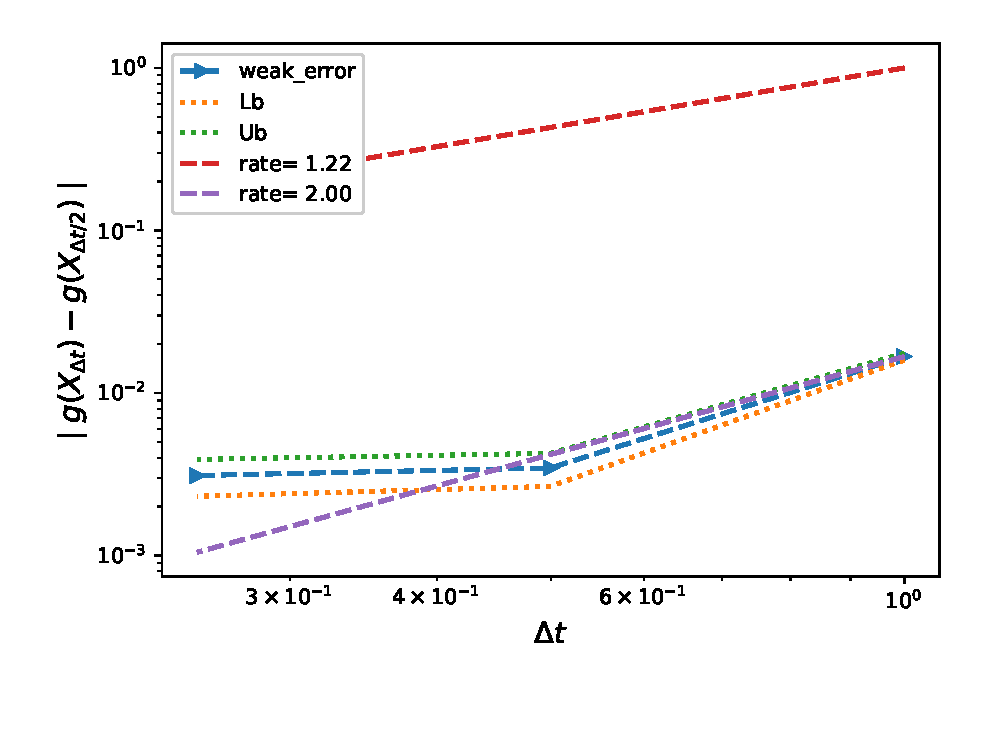
\includegraphics[width=1\linewidth]{./figures/weak_error_rates_basket_2d/with_richardson/weak_convergence_order_differences_basket_option_2d_1_richardson_relative_M_4_10_7_plain}
%		\caption{}
%		\label{fig:sub4}
%	\end{subfigure}
%	
%	\caption{The rate of convergence of the weak error for the  Basket ($2$-dimensional) call option with Richardson extraploation (level 1), using MC with $M=4.10^7$: a)   b) $\abs{\expt{3 g(X_{\Delta t/2})-g(X_{\Delta t})-2 g(X_{\Delta t/4})}}$}
%	\label{fig:Weak_rate_call_with_rich_level1}
%\end{figure}




\FloatBarrier
\subsubsection{Comparing relative errors}\label{sec:Comparing relative errors, basket call}
\subsubsection*{Without Richardson extrapolation}


\begin{table}[h!]
\centering
\begin{tabular}{l*{6}{c}r}
Method \textbackslash  Steps            & $2$ & $4$ & $8$ & $16$ &   \\
\hline
MISC ($TOL_{\text{MISC}}=5.10^{-1},\beta=16$)  & $
 13.0009$ & $    12.8577$ & $    12.8854$ & $
   12.9000$  \\
MISC ($TOL_{\text{MISC}}=10^{-1},\beta=16$)  & $
 13.0009$ & $   12.9912
$ & $
12.9556
$ &$ 12.9231$  \\
MISC ($TOL_{\text{MISC}}=5.10^{-2},\beta=16$) & $
 13.0009$ & $    13.0049
$ & $ 12.9550

$ & $-$  \\
MISC ($TOL_{\text{MISC}}=10^{-2},\beta=16$) & $  13.0548$ & $    13.0046$ & $   12.9550
$ &$-$  \\
%MISC ($TOL_{\text{MISC}}=10^{-3},\beta=16$) & $   13.0548$ & $   13.0046$ & $-$ & $-$  \\
%MISC ($TOL_{\text{MISC}}=10^{-4},\beta=16$) & $  13.0545$ & $   13.0047$ & $-$ & $-$  \\
%MISC ($TOL_{\text{MISC}}=10^{-5},\beta=16$) & $  13.0545$ & $-$ & $-$ & $-$  \\
\hline
MC method ($M=4.10^{7}$)   & $  13.0203
$ & $ 12.9969$ & $12.9301
$ & $ 12.9194 $  \\
\hline
\end{tabular}
\caption{Basket ($2$-dimensional) call option price of the different methods for different number of time steps, without Richardson extrapolation.}
\label{table:Basket 2d option price of the different methods for different number of time steps, without Richardson extrapolation, beta_16}
\end{table}







\FloatBarrier



\begin{table}[h!]
	\centering
	\begin{tabular}{l*{6}{c}r}
		Method \textbackslash  Steps            & $2$ & $4$ & $8$ & $16$  \\
		\hline
		MC Bias ($M=4.10^{7}$)  & 	$ \underset{(      0.1195
			 )}{\mathbf{0.0093}}$  & $\underset{(0.0968
			 )}{\mathbf{ 0.0075
		}}$  & $\underset{(  0.0297)}{\mathbf{0.0023}}$ & $\underset{(         0.0181
	
			)}{\mathbf{  0.0014 }}$\\ 
		
		MC Statistical error  ($M=4.10^{7}$)   & 	$ \underset{( 3.2e-03  )}{\mathbf{2.5e-04}}$  & $\underset{(3.5e-03 )}{\mathbf{ 2.7e-04
		}}$  & $\underset{(3.6e-03 )}{\mathbf{2.8e-04}}$ & $\underset{( 3.6e-03 )}{\mathbf{ 2.8e-04  }}$\\ 
		\hline
	\end{tabular}
	\caption{Bias and statistical errors of MC  for computing Basket ($2$-dimensional) call option price  for different number of time steps, without Richardson extrapolation. The numbers between parentheses are the corresponding absolute errors.}
	\label{Bias and Statistical errors of MC  for computing Basket 2d Call option price  for different number of time steps, without Richardson extrapolation. The numbers between parentheses are the corresponding absolute errors.}
\end{table}


\FloatBarrier
\begin{table}[h!]
\centering
\begin{tabular}{l*{6}{c}r}
Method \textbackslash  Steps            & $2$ & $4$ & $8$ & $16$  \\
\hline
MISC ($TOL_{\text{MISC}}=5.10^{-1}$)  & $\underset{(  0.0194)}{\mathbf{    0.0015}}$  & $\underset{(   0.1392
	)}{\mathbf{    0.0108}}$ & $\underset{( 0.0447
	
	-
	)}{\mathbf{ 0.0035}}$ &$\underset{(
	0.0194)}{\mathbf{   \red{ 0.0015}}}$ \\
MISC ($TOL_{\text{MISC}}=10^{-1}$)  & $\underset{(  0.0194)}{\mathbf{    0.0015}}$   & $\underset{(   0.0057)}{\mathbf{4.4e-04}}$ & $\underset{(0.0255)}{\mathbf{\red{0.0020}}}$ &$\underset{(0.0037)}{\mathbf{2.9e-04}}$ \\
MISC ($TOL_{\text{MISC}}=5.10^{-2}$)  & $\underset{(  0.0194)}{\mathbf{    0.0015}}$  & $\underset{( 0.0080)}{\mathbf{\red{6.2e-04}}}$ & $\underset{(
	0.0249
	)}{\mathbf{0.0019}}$ &$\underset{(-)}{\mathbf{-}}$ \\
MISC ($TOL_{\text{MISC}}=10^{-2}$)  & $\underset{( 0.0345)}{\mathbf{\red{0.0027}}}$  & $\underset{( 0.0077)}{\mathbf{6.0e-04}}$ & $\underset{(
	0.0249
	)}{\mathbf{0.0019}}$&$\underset{(-)}{\mathbf{-}}$ \\
%MISC ($TOL_{\text{MISC}}=10^{-3}$)  & $\underset{( 0.0345)}{\mathbf{0.0027}}$  & $\underset{( 0.0077)}{\mathbf{6.0e-04}}$ & $\underset{(
%-
%	)}{\mathbf{-}}$ &$\underset{(-)}{\mathbf{-}}$ \\
%MISC ($TOL_{\text{MISC}}=10^{-4}$)  & $\underset{( 0.0342)}{\mathbf{0.0027
%}}$  & $\underset{( 0.0078)}{\mathbf{6.0e-04}}$& $\underset{(
%	-
%	)}{\mathbf{-}}$ &$\underset{(-)}{\mathbf{-}}$ \\
%MISC ($TOL_{\text{MISC}}=10^{-5}$)  & $\underset{( 0.0342)}{\mathbf{0.0027
%}}$  & $\underset{( -)}{\mathbf{-}}$ & $\underset{(
%	-
%	)}{\mathbf{-}}$ &$\underset{(-)}{\mathbf{-}}$ \\
\hline
\end{tabular}
\caption{Quadrature error of MISC, with different tolerances, to compute Basket ($2$-dimensional) call option price  for different number of time steps, without Richardson extrapolation. The numbers between parentheses are the corresponding absolute errors. The values marked in red correspond to stable quadrature errors for MISC, and will be used for complexity comparison against MC.}
\label{Quadrature error of MISC to compute Basket 2d Call option price of the different tolerances for different number of time steps, without Richardson extrapolation. The numbers between parentheses are the corresponding absolute errors, beta_16}
\end{table}

\FloatBarrier
	\begin{figure}[h!]
	\centering
	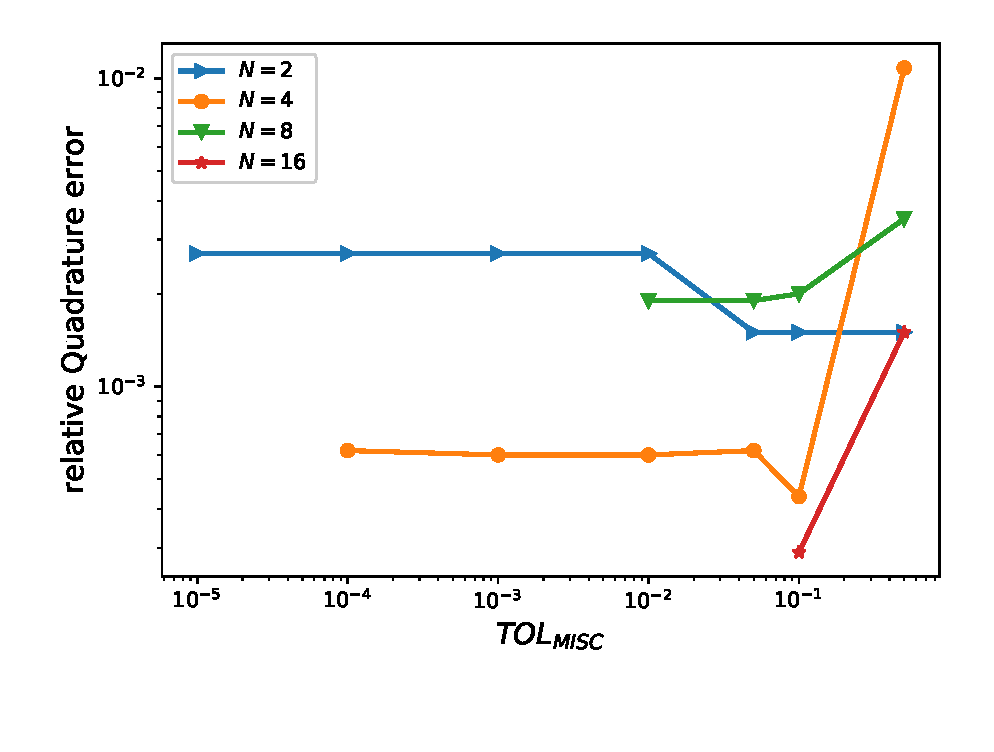
\includegraphics[width=0.4\linewidth]{./figures/Basket_2d_MISC_quadrature_error/relative_quad_error_wrt_MISC_TOL_non_rich}
	
	
	\caption{Relative quadrature error of MISC,with different tolerances,  to compute Basket ($2$-dimensional) call option price for different number of time steps, without Richardson extrapolation.}
	\label{fig:Quadrature_error_non_rich_basket_Call}
\end{figure}

\FloatBarrier

\begin{table}[h!]
	\centering
	\begin{tabular}{l*{6}{c}r}
		Method \textbackslash  Steps            & $2$ & $4$ & $8$ & $16$  \\
		\hline
		MISC ($TOL_{\text{MISC}}=5.10^{-1}$) &$\mathbf{0.0108}$ & $\mathbf{0.0183}$ & $\mathbf{0.0058}$ & $\mathbf{\red{0.0029}}$  \\	
		MISC ($TOL_{\text{MISC}}=10^{-1}$) & $\mathbf{0.0108}$ & $\mathbf{0.0079}$ & $\mathbf{\red{0.0043}}$ & $\mathbf{0.0017}$  \\	
		MISC ($TOL_{\text{MISC}}=5.10^{-2}$) & $\mathbf{0.0108}$ & $\mathbf{\red{0.0081}}$ & $\mathbf{0.0042}$ & $\mathbf{-}$  \\	
		MISC ($TOL_{\text{MISC}}=10^{-2}$)& $\mathbf{\red{0.0120}}$ & $\mathbf{0.0081}$ &$\mathbf{0.0042}$ & $\mathbf{-}$  \\	
%		MISC ($TOL_{\text{MISC}}=10^{-3}$) &  $\mathbf{0.0120}$& $\mathbf{0.0081}$ & $\mathbf{-}$ & $\mathbf{-}$  \\	
%		MISC ($TOL_{\text{MISC}}=10^{-4}$) &  $\mathbf{0.0120}$& $\mathbf{0.0081}$ & $\mathbf{-}$ & $\mathbf{-}$  \\
%		MISC ($TOL_{\text{MISC}}=10^{-5}$) &  $\mathbf{0.0120}$& $\mathbf{-}$ & $\mathbf{-}$ & $\mathbf{-}$  \\
		\hline	
		MC +root finding  & $\mathbf{\red{0.0120}}$ & $\mathbf{\red{0.0081}}$ & $\mathbf{\red{0.0042}}$ & $\mathbf{\red{0.0029}}$\\
		MC   &  $\mathbf{\red{0.0119}}$ & $\mathbf{\red{0.0081}}$ & $\mathbf{\red{0.0042}}$ & $\mathbf{\red{0.0029}}$  \\	
		\hline
	\end{tabular}
	\caption{Total relative  error of MISC, with different tolerances, and MC to compute Basket ($2$-dimensional) call option price  for different number of time steps, without Richardson extrapolation.  The values marked in red, for MISC method, correspond to the total relative errors associated with  stable quadrature errors for MISC, and will be used for complexity comparison against MC.}
	\label{Total error of MISC and MC to compute Basket 2dCall option price of the different tolerances for different number of time steps, without Richardson extrapolation. The numbers between parentheses are the corresponding absolute errors,beta_16}
\end{table}

\FloatBarrier

\begin{table}[h!]
\centering
\begin{tabular}{l*{6}{c}r}
Method \textbackslash  Steps            & $2$ & $4$ & $8$ & $16$ &   \\
\hline
MISC ($TOL_{\text{MISC}}=5.10^{-1}$) & $3$ & $15$ & $197$ & $\red{ 1048}$  \\
MISC ($TOL_{\text{MISC}}=10^{-1}$)  & $3$ & $34$ & $\red{217}$ & $ 7324$  \\
MISC ($TOL_{\text{MISC}}=5.10^{-2}$)  & $3$ & $\red{44}$ & $917$ & $-$  \\
MISC ($TOL_{\text{MISC}}=10^{-2}$)  & $\red{4}$ & $98$ & $1825$ & $-$  \\
%MISC ($TOL_{\text{MISC}}=10^{-3}$)   & $4$ & $245$ & $-$ & $-$  \\
%MISC ($TOL_{\text{MISC}}=10^{-4}$)   & $23$ & $1035$ & $-$ & $-$  \\
%MISC ($TOL_{\text{MISC}}=10^{-5}$)   & $58$ & $-$ & $-$ & $-$  \\
\hline
MC method +root finding   & $\red{  557}$ & $\red{   13564}$ & $\red{  1218}$ & $\red{ 1749
}$  \\
MC method & $\red{164}$ & $\red{3518}$ & $\red{451}$ & $\red{1112}$  \\
\hline

Ratio of	$\text{(MC+root finding)}/\text{(MISC)}$ & $\red{139}$ & $\red{  308}$ & $\red{5.6}$ & $\red{1.7}$  \\
Ratio of	$(\text{MC})/(\text{MISC})$ & $\red{41}$ & $\red{80}$ & $\red{2.1}$ & $\red{ 1.1}$  \\
\hline
\end{tabular}
\caption{Comparison of the computational time of  MC and MISC, used to compute Basket ($2$-dimensional) call option price  for different number of time steps, without Richardson extrapolation. The average computational time of MC is computed over $10$ runs.}
\label{Comparsion of the computational time of  MC and MISC, used to compute Basket 2d Call option price  for different number of time steps, without Richardson extrapolation, beta_16}
\end{table}


\FloatBarrier

\begin{figure}[h!]
	\centering
	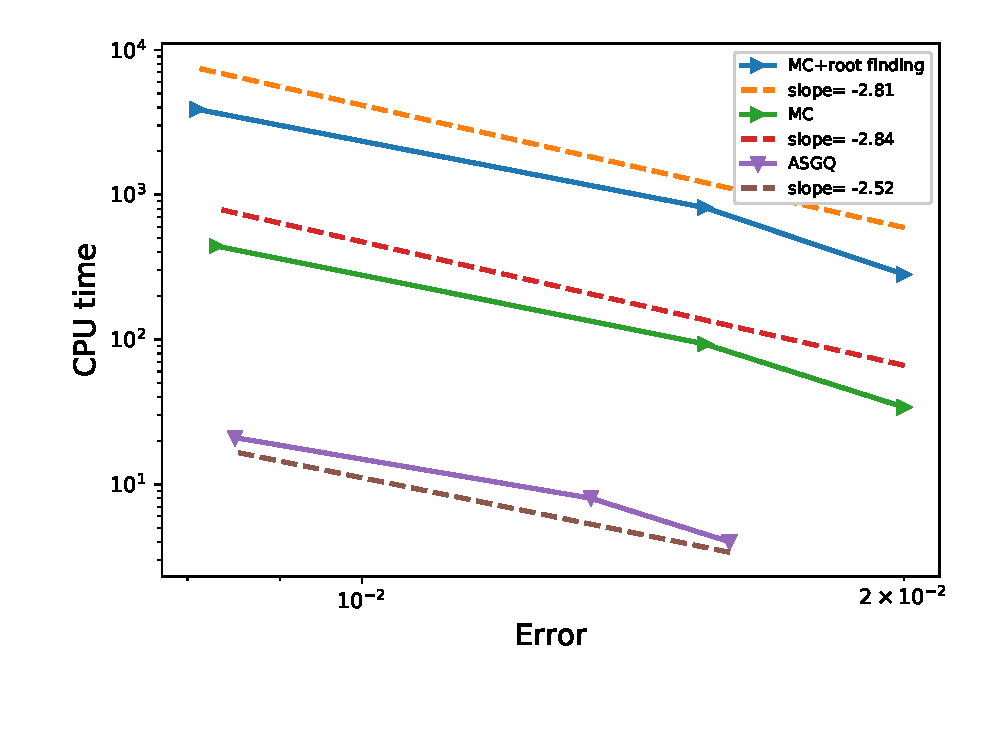
\includegraphics[width=0.4\linewidth]{./figures/Basket_2d_Complexity_rates/error_vs_time}
	
	\caption{Complexity plot for MC and MISC for the case without Richardson extrapolation.}
	\label{fig:Complexity plot for MC and MISC , Basket 2d Call non rich}
\end{figure}

\FloatBarrier
%\subsubsection*{With Richardson extrapolation (level $1$)}
%
%\FloatBarrier
%
%
%\begin{table}[h!]
%	\centering
%	\begin{tabular}{l*{6}{c}r}
%		Method \textbackslash  Steps            & $1-2$ & $2-4$ & $4-8$  \\
%		\hline
%		MISC ($TOL_{\text{MISC}}=5.10^{-1}$, $\beta=16$) & $   13.0821
%		$ & $ 12.7353
%		$ & $   12.8138$   \\
%		MISC ($TOL_{\text{MISC}}=10^{-1}$, $\beta=16$)  & $    13.1898
%		$ & $ 12.8791
%		$ & $   12.9055$  \\
%		MISC ($TOL_{\text{MISC}}=5.10^{-2}$, $\beta=16$) & $    13.1898
%		$ & $ 12.9151 $ & $-$   \\
%		MISC ($TOL_{\text{MISC}}=10^{-2}$,$\beta=16$ ) & $    13.1898
%		$ & $ 
%		12.9567$ & $-$  \\
%%		MISC ($TOL_{\text{MISC}}=10^{-3}$, $\beta=16$) & $    13.1898
%%		$ & $ 12.9558$ & $-$ \\
%%			MISC ($TOL_{\text{MISC}}=10^{-4}$,$\beta=16$) & $  13.1893
%%			  
%%		$ & $-$ & $-$  \\
%		\hline
%		MC method ($M=4.10^{7}$)   & $ 13.1927$ & $12.9768$ & $12.9322$ \\
%		\hline
%	\end{tabular}
%	\caption{Basket $2$-dimensional call option price of the different methods for different number of time steps, with Richardson extrapolation (level $1$).}
%	\label{table: Call option price of the different methods for different number of time steps, with Richardson extrapolation (level1),beta_16}
%\end{table}
%
%\FloatBarrier
%
%\begin{table}[h!]
%	\centering
%	\begin{tabular}{l*{6}{c}r}
%		Method \textbackslash  Steps            & $1-2$ & $2-4$ & $4-8$ & $8-16$  \\
%		\hline
%		MC Bias ($M=4.10^7$)   & 	$ \underset{(    0.2919
%			
%			)}{\mathbf{0.0226}}$  & $\underset{(    0.0760)}{\mathbf{ 0.0059
%		}}$  & $\underset{(   0.0314)}{\mathbf{0.0024}}$ & $\underset{( 0.0085
%	
%			)}{\mathbf{ 0.0007}}$\\ 
%		
%		MC Statistical error ($M=4.10^7$)     & 	$ \underset{(  3.7e-03 )}{\mathbf{2.9e-04}}$  & $ \underset{(  3.7e-03 )}{\mathbf{2.9e-04}}$ & $ \underset{(  3.7e-03 )}{\mathbf{2.9e-04}}$ & $ \underset{(  3.6e-03 )}{\mathbf{2.8e-04}}$\\ 
%		
%		\hline
%	\end{tabular}
%	\caption{Bias and statistical errors of MC  for computing Basket ($2$-dimensional) call option price  for different number of time steps, with Richardson extrapolation (level $1$). The numbers between parentheses are the corresponding absolute errors.}
%	\label{Bias and Statistical errors of MC  for computing Basket ($2$-dimensional) Call option price  for different number of time steps, with Richardson extrapolation (level $1$). The numbers between parentheses are the corresponding absolute errors,beta_16}
%\end{table}
%
%\FloatBarrier
%
%\begin{table}[h!]
%	\centering
%	\begin{tabular}{l*{6}{c}r}
%		Method \textbackslash  Steps            & $1-2$ & $2-4$ & $4-8$   \\
%		\hline
%		MISC ($TOL_{\text{MISC}}=5.10^{-1}$)  & $\underset{(0.1106)}{\mathbf{0.0086
%		}}$ & $\underset{(0.2415)}{\mathbf{0.0187}}$& $\underset{(
%		    0.1184
%		
%			)}{\mathbf{ 0.0092}}$  \\
%		MISC ($TOL_{\text{MISC}}=10^{-1}$)  & $\underset{(0.0029)}{\mathbf{\red{0.0002}
%		}}$  & $\underset{(     0.0977
%	 )}{\mathbf{      0.0076}}$& $\underset{(
%		    0.0267
%		
%			)}{\mathbf{   \red{0.0021}}}$  \\
%		MISC ($TOL_{\text{MISC}}=5.10^{-2}$) & $\underset{(0.0029)}{\mathbf{0.0002
%		}}$ & $\underset{(    0.0617)}{\mathbf{  0.0048}}$& $\underset{(
%			-
%			)}{\mathbf{-}}$  \\
%		MISC ($TOL_{\text{MISC}}=10^{-2}$)  & $\underset{(0.0029)}{\mathbf{0.0002
%		}}$ & $\underset{(  0.0201)}{\mathbf{   \red{0.0016}}}$& $\underset{(
%			-
%			)}{\mathbf{-}}$ \\
%%		MISC ($TOL_{\text{MISC}}=10^{-3}$)  & $\underset{(0.0029)}{\mathbf{0.0002
%%		}}$  & $\underset{(    0.0210
%%	)}{\mathbf{   0.0016}}$& $\underset{(
%%			-
%%			)}{\mathbf{-}}$  \\
%%		MISC ($TOL_{\text{MISC}}=10^{-4}$)  & $\underset{(0.0029)}{\mathbf{0.0002
%%		}}$ & $\underset{(-)}{\mathbf{-}}$& $\underset{(
%%			-
%%			)}{\mathbf{-}}$  \\
%	
%		\hline
%	\end{tabular}
%	\caption{Quadrature error of MISC, with different tolerances,  to compute Basket ($2$-dimensional) call option price for different number of time steps, with Richardson extrapolation. The numbers between parentheses are the corresponding absolute errors. The values marked in red correspond to stable quadrature errors for MISC, and will be used for complexity comparison against MC.}
%	\label{Quadrature error of MISC to compute Basket 2d Call option price of the different tolerances for different number of time steps, with Richardson extrapolation. The numbers between parentheses are the corresponding absolute errors, beta_16}
%\end{table}
%
%
%
%
%\FloatBarrier
%\begin{table}[h!]
%	\centering
%	\begin{tabular}{l*{6}{c}r}
%		Method \textbackslash  Steps            & $1-2$ & $2-4$ & $4-8$   \\
%		\hline
%		MISC ($TOL_{\text{MISC}}=5.10^{-1}$) & $\mathbf{0.0312}$& $\mathbf{0.0246}$ & $\mathbf{0.0116}$  \\
%		MISC ($TOL_{\text{MISC}}=10^{-1}$) & $\mathbf{\red{0.0228}}$& $\mathbf{0.0135}$ & $\mathbf{\red{0.0045}}$   \\	
%		MISC ($TOL_{\text{MISC}}=5.10^{-2}$) & $\mathbf{0.0228}$& $\mathbf{0.0107}$ & $\mathbf{-}$   \\
%		MISC ($TOL_{\text{MISC}}=10^{-2}$)& $\mathbf{0.0228}$& $\mathbf{\red{0.0075}}$ & $\mathbf{-}$   \\	
%%		MISC ($TOL_{\text{MISC}}=10^{-3}$) & $\mathbf{0.0228}$& $\mathbf{0.0075}$ & $\mathbf{-}$ \\
%%		MISC ($TOL_{\text{MISC}}=10^{-4}$) & $\mathbf{0.0228}$& $\mathbf{-}$ & $\mathbf{-}$  \\
%		\hline	
%		MC +root finding & $\mathbf{\red{-}}$ & $\mathbf{\red{-}}$ & $\mathbf{\red{-}}$   \\	
%		MC   &  $\mathbf{\red{-}}$ & $\mathbf{\red{-}}$ & $\mathbf{\red{-}}$   \\	
%		\hline
%	\end{tabular}
%	\caption{Total relative error of MISC, with different tolerances, and MC to compute Basket ($2$-dimensional) call option price  for different number of time steps, with Richardson extrapolation.  The values marked in red, for MISC method, correspond to the total relative errors associated with  stable quadrature errors for MISC, and will be used for complexity comparison against MC.}
%	\label{Total error of MISC and MC to compute Basket 2dCall option price of the different tolerances for different number of time steps, with Richardson extrapolation. The numbers between parentheses are the corresponding absolute errors,beta_16}
%\end{table}
%\FloatBarrier
%\begin{table}[h!]
%	\centering
%	\begin{tabular}{l*{6}{c}r}
%		Method \textbackslash  Steps            & $1-2$ & $2-4$ & $4-8$     \\
%		\hline
%		MISC ($TOL_{\text{MISC}}=5.10^{-1}$) & $5$  & $39$ & $396$  \\
%		MISC ($TOL_{\text{MISC}}=10^{-1}$)  & $\red{8}$  & $70$ & $ \red{1379}$  \\
%		MISC ($TOL_{\text{MISC}}=5.10^{-2}$)  & $8$  & $76$ & $-$   \\
%		MISC ($TOL_{\text{MISC}}=10^{-2}$) & $8$  & $ \red{262}$ & $-$ \\
%%		MISC ($TOL_{\text{MISC}}=10^{-3}$)   & $8$  & $339$ & $-$   \\
%%		MISC ($TOL_{\text{MISC}}=10^{-4}$)   & $55$  & $-$ & $-$   \\
%		\hline
%		
%		\hline
%	\end{tabular}
%	\caption{Comparison of the computational time of  MISC, used to compute Basket $2$-dimensional call option price  for different number of time steps, with Richardson extrapolation (level $1$). The average computational time of MC is computed over $10$ runs.}
%	\label{Comparsion of the computational time of  MC and MISC, used to compute Call option price  for different number of time steps, with Richardson extrapolation (level $1$),beta_16}
%\end{table}
%\FloatBarrier
%
%%\subsubsection{Case of  $3$-dimensional Basket call option}
%%\subsubsection*{Weak error plots} \label{sec:Weak error plots_Basket_3D_call}
%%
%%\begin{figure}[h!]
%%	\centering
%%	\begin{subfigure}{.35\textwidth}
%%		\centering
%%		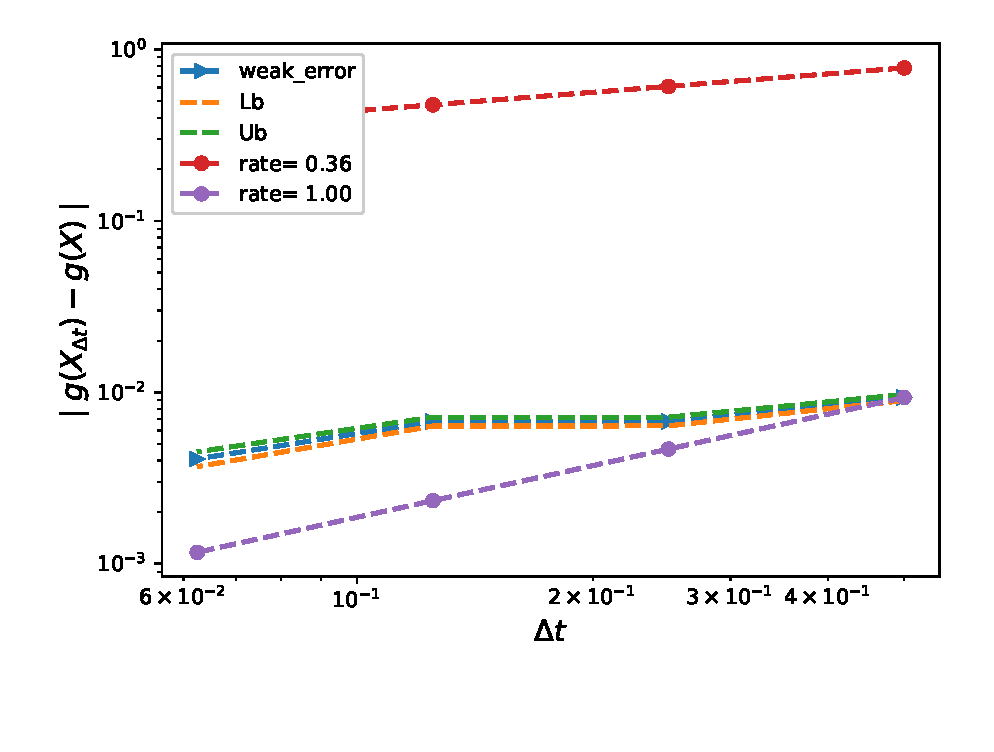
\includegraphics[width=1\linewidth]{./figures/weak_error_rates_basket_3d/without_richardson/weak_convergence_order_basket_option_3d_1_relative_M_7_10_7_plain_1}
%%		\caption{}
%%		\label{fig:sub3}
%%	\end{subfigure}%
%%	\begin{subfigure}{.35\textwidth}
%%		\centering
%%		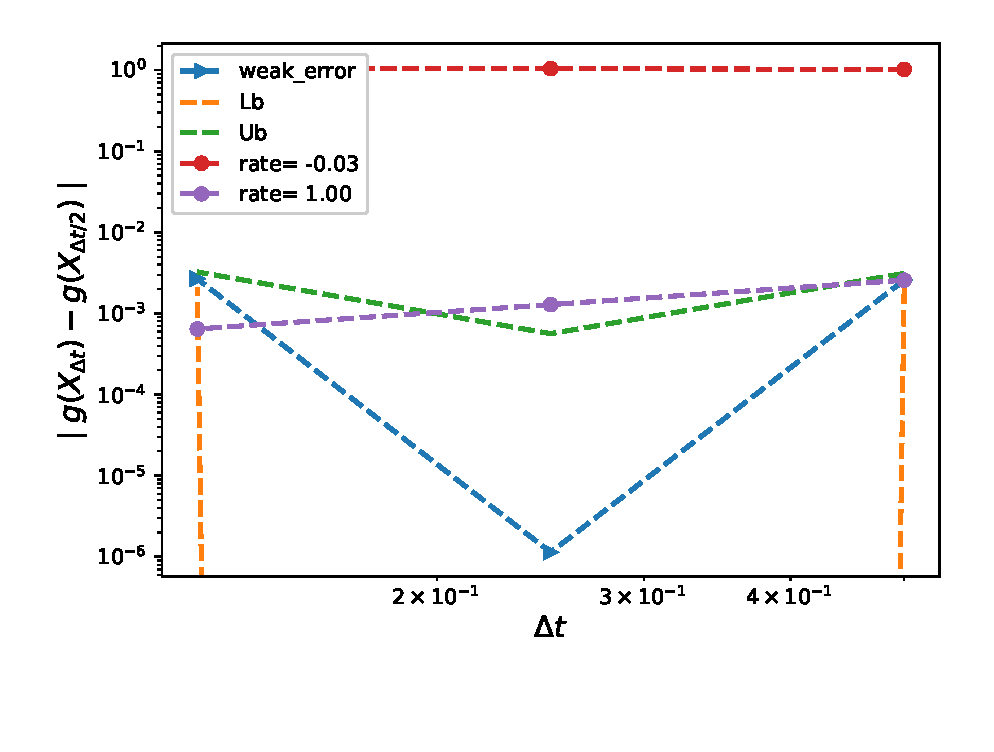
\includegraphics[width=1\linewidth]{./figures/weak_error_rates_basket_3d/without_richardson/weak_convergence_order_differences_basket_option_3d_1_relative_M_7_10_7_plain_1}
%%		\caption{}
%%		\label{fig:sub4}
%%	\end{subfigure}
%%	
%%	\caption{The rate of convergence of the weak error for the Basket ($3$-dimensional) call option, without Richardson extraploation, using MC with $M=7.10^7$: a) $\abs{\expt{g(X_{\Delta t})}-g(X)}$  b) $\abs{\expt{g(X_{\Delta t})-g(X_{\Delta t/2})}}$ }
%%	\label{fig:Weak_rate_basket_3d_without_rich}
%%\end{figure}
%%\FloatBarrier
%%
%%\subsubsection*{Comparing relative errors}\label{sec:Comparing relative errors, basket_3d call}
%%\subsubsection*{Without Richardson extrapolation}
%%
%%
%%\begin{table}[h!]
%%	\centering
%%	\begin{tabular}{l*{6}{c}r}
%%		Method \textbackslash  Steps            & $2$ & $4$ & $8$ & $16$ &   \\
%%		\hline
%%		MISC ($TOl=5.10^{-1},\beta=16$)  & $-$ & $-$ & $-$ & $-$  \\
%%		MISC ($TOl=10^{-1},\beta=16$)   & $-$ & $-$ & $-$ & $-$  \\
%%		MISC ($TOl=5.10^{-2},\beta=16$) & $-$ & $-$ & $-$ & $-$  \\
%%		MISC ($TOl=10^{-2},\beta=16$) & $-$ & $-$ & $-$ & $-$  \\
%%		MISC ($TOl=10^{-3},\beta=16$)  & $-$ & $-$ & $-$ & $-$  \\
%%		MISC ($TOl=10^{-4},\beta=16$)  & $-$ & $-$ & $-$ & $-$  \\
%%		MISC ($TOl=10^{-5},\beta=16$)  & $-$ & $-$ & $-$ & $-$  \\
%%		\hline
%%		MC method ($M=7.10^{7}$)    & $-$ & $-$ & $-$ & $-$  \\
%%		\hline
%%	\end{tabular}
%%	\caption{Basket ($3$-dimensional) Call option price of the different methods for different number of time steps, without Richardson extrapolation.}
%%	\label{table:Basket 3d option price of the different methods for different number of time steps, without Richardson extrapolation, beta_}
%%\end{table}
%%
%%
%%
%%
%%
%%
%%\begin{table}[h!]
%%	\centering
%%	\begin{tabular}{l*{6}{c}r}
%%		Method \textbackslash  Steps            & $2$ & $4$ & $8$ & $16$ &   \\
%%		\hline
%%		MISC ($TOl=5.10^{-1}$)  & $-$ & $-$ & $-$ & $-$  \\
%%		MISC ($TOl=10^{-1}$)   & $-$ & $-$ & $-$ & $-$  \\
%%		MISC ($TOl=5.10^{-2}$)   & $-$ & $-$ & $-$ & $-$  \\
%%		MISC ($TOl=10^{-2}$) & $-$ & $-$ & $-$ & $-$  \\
%%		MISC ($TOl=10^{-3}$)   & $-$ & $-$ & $-$ & $-$  \\
%%		MISC ($TOl=10^{-4}$)   & $-$ & $-$ & $-$ & $-$  \\
%%		MISC ($TOl=10^{-5}$)   & $-$ & $-$ & $-$ & $-$  \\
%%		\hline
%%		MC method +root finding   & $-$ & $-$ & $-$ & $-$  \\
%%		MC method  & $-$ & $-$ & $-$ & $-$  \\
%%		\hline
%%		
%%		Ratio of	$\text{(MC+root finding)}/\text{(MISC)}$  & $-$ & $-$ & $-$ & $-$  \\
%%		Ratio of	$(\text{MC})/(\text{MISC})$ & $-$ & $-$ & $-$ & $-$  \\
%%		\hline
%%	\end{tabular}
%%	\caption{Comparison of the computational time of  MC and MISC, used to compute Basket ($3$-dimensional) Call option price  for different number of time steps, without Richardson extrapolation}
%%	\label{Comparsion of the computational time of  MC and MISC, used to compute Basket 3d Call option price  for different number of time steps, without Richardson extrapolation, beta_16}
%%\end{table}
%

